%%% One-side print:
\documentclass[11pt,a4paper]{report}
\usepackage[top=25mm,bottom=25mm,right=25mm,left=30mm,head=12.5mm,foot=12.5mm]{geometry}
\let\openright=\clearpage

\usepackage{tikz}
\usetikzlibrary{shapes.geometric, arrows}

\usepackage{ifthen}
\usepackage{caption} % sources in captions
\newcommand{\source}[1]{\caption*{ \raggedleft \textit{Source{#1}}} }

% poznámky enviroment
\newenvironment{koment}%
        {%
            \ifthenelse{\isundefined{\showtodos}}%
                    {\expandafter\comment}%
                    {\par \centering \color{blue}{} \em }%
                    }%
         {%
            \ifthenelse{\isundefined{\showtodos}}%
                    {\expandafter\endcomment}%
                    {\par \centering \color{blue}{}%
                    }%
          }


\newcommand{\showtodos}{} %zakomentovat pro skrytí poznámek! #TODO

\usepackage{pgfplots} %% tikz pro kresleni grafu

% \usepackage{natbib} %% hraju si s citacema 

% priklady: 
    % citeauthor*{jon90} --> Jones, Baker, and Williams
    
    % \citet*{jon90} --> Jones, Baker, and Williams (1990)
    
    % \citep*{jon90} --> (Jones, Baker, and Williams, 1990)
    
    % \citealt{jon90} --> Jones, Baker, and Williams, 1990

% workaround: 

% \newcommand{\citet}[1]{\citeauthor{#1} \shortcite{#1}}
% \newcommand{\citep}{\cite}
% \newcommand{\citealp}[1]{\citeauthor{#1} \citeyear{#1}}


%%% Two-side print:
%\documentclass[11pt,a4paper,twoside,openright]{report}
%\usepackage[top=25mm,bottom=25mm,right=25mm,left=30mm,head=12.5mm,foot=12.5mm]{geometry}
%\let\openright=\cleardoublepage

%%% DEFINITION OF BASIC VARIABLES
\def\TypPrace{BP}                % bakalářská práce/bachelor thesis
%\def\TypPrace{DP}               % diplomová práce/master thesis
%\def\Jazyk{cze}                  % čeština/czech
%\def\Jazyk{slo}                 % slovenština/slovak
\def\Jazyk{eng}                 % angličtina/english

%%% Definition of some useful macros
\input{makra}

%%% Název práce v jazyce práce (přesně podle zadání)
%%% Title of the thesis in the language used in the text (exact according to assignment)
\def\NazevPrace{Benford’s Law and the Statistical Detection of Election Fraud}

%%% Jméno autora
%%% Author's name - First name Surname
\def\AutorPrace{Kristýna Bednářová}

%%% Rok odevzdání a měsíc (slovně)
%%% Year of submission and month (verbally) - month YYYY
\def\DatumOdevzdani{May 2025}

%%% Vedoucí práce: Jméno a příjmení s~tituly
%%% Supervisor: First name and surname with titles
\def\Vedouci{Mgr. Jana Cibulková, Ph.D.}

%%% Konzultant práce: Jméno a příjmení s~tituly
%%% Consultant: First name and surname with titles
\def\Konzultant{} %full consultant’s name (incl. degrees)

%%% Studijní program
%%% Study program
\def\StudijniProgram{Mathematical Methods in Economics}

%%% Studijní program - specializace
%%% Study program - specialization
\def\Specializace{Data Analyses and Modeling}

%%% Nepovinné poděkování (vedoucímu práce, konzultantovi, tomu, kdo zapůjčil software, literaturu apod.)
%%% Optional thanks (the supervisor, the consultant, the borrower of software, literature, etc.)
\def\Podekovani{%
Thanks.
}

%%% Abstract (recommended range of about 150-250 words; this is not a thesis assignment)
\def\Abstrakt{%
Abstract.
}
\def\KlicovaSlova{keyword, important term, another topic, and another one}


%%% Titulní strana a různé povinné informativní strany
%%% Title page and various mandatory information pages
\begin{document}

\include{beginning}

%%% Strana s automaticky generovaným obsahem práce
%%% A page with automatically generated content of the thesis
\setcounter{tocdepth}{2}
\tableofcontents

%%% Seznam obrázků v práci
%%% List of figures in the thesis
\openright
\listoffigures

Note: The list of figures should be used if the number of figures in the text is more than 20.

%%% Seznam tabulek v práci (volitelně)
%%% List of tables in the thesis (optionally)
\clearpage
\listoftables

Note: The list of tables should be used if the number of tables in the text is more than 20.  

%%% Seznam zdrojových kódů v práci (volitelně)
%%% List of source listings in the thesis (optionally)
\clearpage
\lstlistoflistings
Note: The list of programme code excerpts should be used if the number of programme codes excerpts in the text is more than 20.

%%% Seznam zkratek v práci (volitelně)
%%% List of abbreviations in the thesis (optionally)
\chapter*{\SeznamZkratek}

\begin{multicols}{2}
\raggedright
\begin{description}
\item [BL] Benford's Law
\item [PDF] Probability Density Function

\end{description}
\end{multicols}

Note: Add a list of abbreviations if the number of abbreviations used in the thesis exceeds 20 and the abbreviations used are not common.


%%% Jednotlivé kapitoly práce jsou pro přehlednost uloženy v samostatných souborech
%%% The individual chapters of the thesis are stored in separate files for clarity

{%
\pagestyle{plain}
%\chapter*{Recommendations for the preparation of thesis at FIS}

\begin{quote}
\bfseries\itshape
This part of the template does not normally belong to the thesis. For the final
text is needed:
\begin{itemize}
\item in file \verb|thesis.tex| delete line \verb|\include{recommendation}|
\item and possibly also an unnecessary file \verb|recommendation.tex|
\end{itemize}
\end{quote}

The following thesis recommendations (hereinafter referred to as 
"recommendations") are intended to evaluate the defensibility of the thesis. 
They are intended for all types of theses in all Bachelor's and Master's degree 
programmes. They are not a substitute for thesis evaluations. If the committee 
considers the thesis undefensible, it should argue that an item in these 
recommendations has not been met.

{\bfseries\sffamily\Large Work done}
\begin{itemize}
\item \vspace*{-2ex}The student has carried out professional work in the field of his/her study programme (including interdisciplinary areas).
\item The final thesis demonstrates the student's orientation in the chosen field and his/her ability to define and achieve the chosen goal in this field. 
\item The student has done professional work of a workload in the range of months.
\end{itemize}

{\bfseries\sffamily\Large Objectives and context}
\begin{itemize}
\item \vspace*{-2ex}The text of the thesis describes the background - the expert context on which the student is based - the situation in professional knowledge or the situation in a specific application case.
\item The starting points contain only the findings that have an impact on the results of the thesis.
\item The text of the thesis clearly describes the aim of the thesis; if the aim is to solve a problem, the problem is sufficiently defined.
\item The reasonableness of the objectives in relation to the baseline is argued.
\item The specificity of the main objective is argued in the text - it is not a generic problem, which has been solved in the same way many times.
\item The formulation of the aim refers to a professional problem, not to the text of the thesis itself, to the reader or to the author. Thus, the objective is not formulated as "to write a text", "to communicate to the reader", "to describe the issue", "to explain", "to become familiar with the literature in the field", etc.
\item The text of the thesis is professional, not popular science. It solves a professional (practical or theoretical) problem.
\end{itemize}

{\bfseries\sffamily\Large Methodology}
\begin{itemize}
\item \vspace*{-2ex}The text of the final thesis describes the process by which the student worked, separately from the results.
\item The procedure is described in steps, from which you can estimate their laboriousness.
\item The procedure lists all the work the student has done. If there are steps in the procedure that the student has not done, they are clearly marked as such (and the reason is given).
\item The procedure is described in such a way that if someone else followed it, they would get similar results as the student.
\item The procedure is described in concrete terms, not just using generic names of thought processes such as analysis, deduction, synthesis, etc.
\item If the procedure used follows established methods described in the literature, it is not necessary to explain their operation in detail. However, the student should justify his/her choice of methods used or describe the deviations of the actual procedure from the established methods.
\end{itemize}

{\bfseries\sffamily\Large Results}
\begin{itemize}
\item \vspace*{-2ex}The results demonstrate that the student has carried out expert work in the field of the study programme (including interdisciplinary areas).
\item From the wording of the text of the final thesis it is clear what is the original result of the student, what is a fact taken from sources and what is speculation or discussion of results.
\item The text describes and interprets the results according to the procedure.
\item The text describes the partial results as outputs of the individual steps. Less important results are presented in the appendices, so that the text remains clear.
\item It is documented that the individual steps (e.g. calculations, descriptive statistics, interview records, program code, researcher's diary, etc.) have been performed, e.g. by uploading attachments to InSIS.
\item The text of the thesis describes the scientific results in a logical flow of argumentation. 
\end{itemize}

{\bfseries\sffamily\Large Conclusions}
\begin{itemize}
\item \vspace*{-2ex}Conclusions assess the degree to which the objective has been met.
\item The conclusions argue how the results have contributed to solving the problem.
\item Conclusions describe the possible impact of the results on the context (situation in the professional environment or in a specific application case), e.g. possible further work.
\item The conclusions mention possible limitations of the results obtained.
\end{itemize}

{\bfseries\sffamily\Large Originality}
\begin{itemize}
\item \vspace*{-2ex}All adopted, translated or paraphrased texts are properly marked and cited in accordance with citation standard APA 7 (we recommend using the Zotero citation tool).
\item In the case of the use of automatic text generation tools, this is in accordance with the rules and methodological recommendations of the Prague University of Economics and Business.
\item The text of the thesis cites and paraphrases only the sources that were used to solve the problem or define the context.
\item The text of the thesis does not unnecessarily recapitulate obvious theoretical knowledge (e.g. from the basic courses of the study programme).
\item In exceptional cases, if the student did not work completely alone, the collaborators (company, academic) and the student's contribution to their performance are indicated at each step of the procedure or in the form of a table in an appendix.
\end{itemize}

{\bfseries\sffamily\Large Form}
\begin{itemize}
\item \vspace*{-2ex}The text of the thesis is written as a coherent structured text, as paragraphs divided into chapters, in a structure suitable for the problem addressed.
\item Pages, tables, figures, appendices (etc.) are numbered.
\item Tables, figures, appendices, program code (etc.) that are not referenced from the body of the text do not appear in the thesis.
\item The format of the thesis is in accordance with the recommendations available on the FIS intranet for students.
\item The final thesis may take the form of a scientific article. In this case, it may be accompanied by an explanatory introduction (e.g. description of the journal, review process, co-authorship of the thesis supervisor, etc.).
\end{itemize}

{\bfseries\sffamily\Large Additional requirements for the thesis}
\begin{itemize}
\item \vspace*{-2ex}The diploma thesis significantly deepens the field of knowledge in the given topic.
\item The thesis clearly specifies the author's own contribution, which is in line with the objectives of the thesis. 
\item It is necessary to validate the results of the thesis (e.g. comparison of the results obtained with the literature, mathematical proof, structured interviews with interest groups, exact testing/measurement of results, etc.).
\end{itemize}

{\bfseries\sffamily\Large Specifics of team theses}
\begin{itemize}
\item \vspace*{-2ex}The fact that the thesis will be carried out in a team must be stated in the Thesis Assignment stored in InSIS and therefore approved by the thesis supervisor and the guarantor of the study programme (specialisation).
\item Each student in the team submits an individual thesis, which is individually assessed, individually defended and evaluated. Each student is responsible for the entire text of the thesis.
\item Only a small part of the thesis may be shared in cases approved by the thesis advisor. More than 70$\%$ of the thesis is individual.
\item The artifacts produced by the team should be published in Git or on the project wiki, for example, and referenced by the authors of the thesis.
\item Each thesis completed by the team includes an appendix entitled Team Members' Contribution to the Result.
\end{itemize}

\chapter*{Introduction}
\addcontentsline{toc}{chapter}{Introduction}

\begin{koment}
In the introduction of the thesis, the author explains why she/he choose the 
chosen topic, thus the \textbf{motivation} of the whole thesis. The introduction must not 
miss the precisely formulated \textbf{main goal} of the thesis (or sub-goals), the 
\textbf{methodology} of the whole thesis (or research questions of hypotheses) should be 
outlined. It is also common practice to outline the \textbf{main results/outcomes} of the 
thesis.

The introduction is followed by individual \textbf{numbered chapters} divided into 
subchapters.

Firstly, an overview of Benford’s Law and its relevance in detecting anomalies in datasets, with a specific focus on its application in electoral data, is provided. A discussion of historical case studies where Benford’s Law has been used will be presented as well.

Next, the statistical techniques and models that will be applied in the analysis of election data are introduced in detail. This includes a description of Benford's Law, its mathematical formulation, and its expected distribution in naturally occurring datasets. Other complementary statistical methods used to strengthen the analysis will also be explained.

Lastly, the methodology will be applied to real election data to assess the presence of anomalies. Detailed steps of the analysis process will be outlined, including data collection, preprocessing, and application of Benford's Law. The results will be discussed, and conclusions will be drawn based on the statistical findings.
\end{koment}

The main objective of this thesis is to analyse election results using Benford's Law and document the whole process along the way. In such process the secondary goal is to detect common errors of other authors and clear out the procedure in which the law should be used with specific focus on analysing election data. 

}


%\chapter{The use of Figures, Tables and Programmes}

The use of tables and graphs/figures in technical text has some common rules and 
some specific ones. We do not present tables and graphs/figures directly in the 
text, but we place them either on separate pages or in a reserved place at the 
top or bottom of regular pages. \LaTeX\ will take care of the placement of 
floating graphs and tables automatically.

Graphs/figures and tables are numbered and equipped with a legend. The legend 
should describe the content of the graph or table in such detail that the reader 
understands them without a thorough study of the text of the work.

There must be a numerical reference to the table and graph/figure in the text (a 
dynamic cross-reference mechanism, which is part of \LaTeX, can be strongly 
recommended). At the appropriate place in the text, we then summarize the most 
important conclusions that can be drawn from a table or graph. The text should 
be legible and understandable even without looking at the tables and graphs, and 
the tables and graphs should be understandable even without reading the text in 
detail.


\section{Figures}

There are several general tips for figures and diagrams.

\begin{itemize}

\item A figure/diagram should be created in the same size as used in the thesis. 
Decreasing a large diagram leads to having unreadable labels. Increasing a small 
diagram leads to poor graphical quality.

\item The diagram axis shall be properly labelled in the thesis language. 
Missing punctuation is tolerable. If a diagram deals with, e.g., weight and 
height, the labels shall say \emph{Height [cm]} and \emph{Weight [kg]}. If the 
graph includes the function \emph{h(x)}, the axes get a label of \emph{x} and 
\emph{h(x)}. Each axis shall bear a clearly defined scale. 

\item If a two-dimensional diagram marks many points, the author should make 
sure that they do not get mixed. If the number of points is too high, the author 
should decrease the size of the symbols that refer to them or select a lower 
number of points to mark in the diagram. Diagrams with thousands of marked 
points cause problems mainly in electronic documents by increasing the file 
size. 

\item If the thesis is to be printed in black and white, the author should avoid 
using colours. Lines should be distinguished by line type (full, dotted, 
dashed…). Sections should be distinguished by distinct shades of grey or 
hatching. The sense of individual line types or hatched sections shall be 
explained either in the diagram textual legend or in a graphic legend integrated 
into the diagram. 

\item Avoid bitmap figures with a low resolution, especially JPEGs. Compression 
artifacts do not look good on paper. 

\end{itemize}

Use the floating environment \verb|figure| to insert images and in addition:
\begin{itemize}
\item for captions use the command \verb|\caption| -- is then also placed in the list of images,
\item The command \verb|\label| is used to identify the image (must always be after the command \verb|\caption|) -- refer to the image in the text with the command \verb|\ref|.
\end{itemize}

\begin{figure}[htbp!]\centering
\includegraphics[width=.66\textwidth]{img/example-fig}
\caption{Frequency of shoe size in the population of men, women and children (CZSO data, Author’s calculation)}
\label{fig:freq-shoe-size}
\end{figure}


\section{Tables}

Use the floating environment \verb|table| to insert tables and in addition:
\begin{itemize}
\item for captions use the command \verb|\caption| -- is then also placed in the list of tables,
\item is used to identify the table using the command \verb|\label| (must always be after the command \verb|\caption|) -- then refer to the table in the text with the command \verb|\ref|.
\end{itemize}

\begin{table}[htbp!]

\centering
%%% Table uses the following packages:
%%% - booktabs (\toprule, \midrule, \bottomrule)
%%% - dcolumn (D column type: centered numbers aligned to
%%% decimal point
%%% Note that there are decimal points in the source code, but
%%% prints commas.

\caption{Maximum plausible estimates of models 1 and 2 (CZSO data, own processing)}\label{tab03:Nejaka}
\begin{tabular}{lrr}
\toprule
 & \multicolumn{1}{c}{\textbf{1}} & \multicolumn{1}{c}{\textbf{2}}\\
\midrule
\multirow{2}{*}{Abs} &$-$10.01*** &42.01**\\
 & (1.01) &(1.89)\\
\multirow{2}{*}{Gender (Male)} & 9.89* & 8.16\\
 & (5.98) &(8.18)\\
Height (cm) & 0.78*** &(0.12) \\
\bottomrule
\multicolumn{3}{p{.45\textwidth}}{\footnotesize \textit{Note:}:
(i) Standard errors obtained based on 500 non-parametric bootstrap iterations are given in parentheses.
(ii) * p < 0.05, ** p < 0.01, *** p < 0.001.}
\end{tabular}
\end{table}

The following tips specifically apply to \textbf{tables}:

\begin{itemize} %% or compactitem from package paralist

\item Never copy tables from statistical software to a thesis. Typically, 
statistical software also includes more information in tables than necessary.

\item Avoid vertical lines. Thicker horizontal lines separate the table from the 
surrounding text, including the legend, weaker horizontal lines separate the 
column headers from the table body, and the individual parts of the table from 
each other. In \LaTeX, the \texttt{booktabs} package implements this form of 
tables. If we want to significantly separate some columns from others, we insert 
a larger space between them

\item Keep the type, format and sense of the field content in a single column. 
It is not advised to enter, e.g., average and percent in the same column.

\item Avoid repeating the same field content too many times. E.g., if the column 
Variance shows the value of 0.5 in the first ten lines and 1.5 in the following 
ten lines, cancel the column. Find a different solution. E.g., one can divide 
the table to two. Alternatively, one can enter descriptive lines that inform of 
a variable value repeating in the following table section. E. g.
\emph{\uv{Variance${}=0,5$}} and below \emph{\uv{Variance${}= 1,5$}}).

\item All numbers shall have the same number of valid digits. Numbers in a table 
shall be aligned to the decimal point.

\item A table sometimes requires the use of abbreviations that do not occur 
elsewhere. Such abbreviations may be explained in the legend or notes below the 
table. Notes below the table may also be used for an explanation of the sense of 
some columns or values.

\end{itemize}


\section{Source codes} 
Algorithms, program listings and description of 
interaction with programs should be distinguished from the rest of the text. One 
possibility is to use {\LaTeX}'s \texttt{listings} package and its environment 
\texttt{lstlistings}.

In the file \texttt{makra.tex} the \texttt{code} environment is defined. Its use looks like this:
\begin{verbatim}
\begin{code}{programming-language}{description}{label-for-ref-ccmmand}
import numpy as np
    
def incmatrix(genl1,genl2):
...
\end{code}
\end{verbatim}

List of supported programming languages: \url{https://www.overleaf.com/learn/latex/Code_listing#Supported_languages}.

For example, the \ref{python-processing} listing is inserted like this:
\begin{verbatim}
\begin{code}{Python}{Sample processing using Python}{python-processing}
...
\end{code}
\end{verbatim}

\begin{code}{Python}{Sample processing using Python}{python-processing}
import numpy as np
    
def incmatrix(genl1,genl2):
    m = len(genl1)
    n = len(genl2)
    M = None #to become the incidence matrix
    VT = np.zeros((n*m,1), int)  #dummy variable
    
    #compute the bitwise xor matrix
    M1 = bitxormatrix(genl1)
    M2 = np.triu(bitxormatrix(genl2),1) 

    for i in range(m-1):
        for j in range(i+1, m):
            [r,c] = np.where(M2 == M1[i,j])
            for k in range(len(r)):
                VT[(i)*n + r[k]] = 1;
                VT[(i)*n + c[k]] = 1;
                VT[(j)*n + r[k]] = 1;
                VT[(j)*n + c[k]] = 1;
                
                if M is None:
                    M = np.copy(VT)
                else:
                    M = np.concatenate((M, VT), 1)
                
                VT = np.zeros((n*m,1), int)
    
    return M
\end{code}

However, the \texttt{listings} package and its environment \texttt{lstlisting} 
offer an almost endless number of configuration parameters, e.g. for syntax 
highlighting of programming languages (several dozen), line numbering, etc.
Examples:


\begin{itemize}
\sloppy
\item \url{https://en.wikibooks.org/wiki/LaTeX/Source_Code_Listings}
\item \url{https://www.overleaf.com/learn/latex/Code_listing#Using_listings_to_highlight_code}
\end{itemize}


\section{Typesetting of mathematics}

We type the variables in italics (\TeX{} does this in math mode itself, but 
don't forget that in the surrounding text and also turn on math mode). We place 
function names upright. For example:
$\textrm{var} (X) = \textsf{E~} X^2 - \bigl(\textsf{E~} X \bigr)^2$.

Fractions inside a paragraph (e. g. $\frac{5}{7}$ or $\frac{x+y}{2}$) they can 
be too cramped, so it's better to bet simple fractions with a slash: $5/7$, 
$(x+y)/2$.

The possibilities of \LaTeX\ for typesetting mathematics are rich, but they may 
not be sufficient in some specific situations. Therefore, American Mathematical 
Society (AMS) packages can be recommended for use. The \texttt{makra.tex} file 
loads the \texttt{amsmath}, \texttt{amsfonts} and \texttt{amsthm} packages 
by default. To penetrate their possibilities, the following will serve:

\begin{itemize}
\item Math Extension with AMS\LaTeX\ -- \url{http://ptgmedia.pearsoncmg.com/images/0321173856/samplechapter/kopkach15.pdf}
\item \url{https://www.overleaf.com/learn/latex/Aligning_equations_with_amsmath}
\item Math Mode -- \url{http://tex.loria.fr/general/Voss-Mathmode.pdf}
\item More Math into LaTeX -- \url{http://tug.ctan.org/info/Math_into_LaTeX-4/Short_Course.pdf}
\end{itemize}

Example of a numbered formula:
\begin{equation}
\mathbf{b}=(\mathbf{X}^\mathsf{T}\mathbf{X})^{-1}\mathbf{X}^\mathsf{T}\mathbf{y}
\end{equation}

Example of unnumbered formulas with functions and indexes:

$$
d_{ij}=\max_{k=1,2,\dots,n} \{d_{ik}+d_{kj}\},
$$
$$
x_{1,2}=b \pm \sqrt{\ln y}.
$$

An example of a formula as part of one paragraph is given on the example of 
supplier capacities in a mathematical model of a traffic problem, which we take 
into account using constraints:
\begin{equation}
\sum_{j=1}^n x_{ij} \le a_i, \qquad i=1,2,\dots,m\ ,
\end{equation}
\noindent
where expression $a_i$ represents capacity of $i$-th supplier.

When deriving a formula by incremental modification, the individual steps are 
usually listed on separate lines (\verb'align*' environment from the \verb|amsmath| package):

\begin{align*}
 f(x) &= (x+a)(x+b) =\\
      &= x^2 + bx + ax + ab =\\
      &= x^2 + (a+b)x + ab
\end{align*}

Example of column adjustment (\verb|eqnarray*|):
\begin{eqnarray*}
\sum_{i=1}^n x_{ij} =1, && j=1,2,\dots,n,\\
\sum_{j=1}^n x_{ij} =1, && i=1,2,\dots,n,\\
u_i + 1 - M(1 - x_{ij}) \le u_j, && i=2,3,\dots,n,\quad j=1,2,\dots,n,\\
u_i \ge 0,              && i=1,2,\dots,n,\\
x_{ij} \in \{0,1\} && i=1,2,\dots,n,\quad j=1,2,\dots,n,\\
\end{eqnarray*}
%\chapter{Bibliography management}

The template assumes the use of This template assumes the use of a bibliographic 
database in \BibTeX\ format for greater flexibility. The use of a bibliographic 
database is not a necessary condition, the standard environment 
\texttt{thebibliography} can also suffice. However, in such a case, it is 
necessary to make interventions in some files, as shown below.

\section{Use of bibliographic database}

\begin{enumerate}

\item \textbf{Package \verb'biblatex', APA-7}\\
The template uses settings via the \verb|biblatex| package to process the 
bibliographic database and also guarantees the use of the \textbf{APA-7} 
citation standard. All settings are listed in the file \texttt{biblatex-setup.tex}.

\item\textbf{Change the database name}\\
The template assumes a database stored in the file \texttt{bibliography.bib}. If 
the database has a different name, then it is necessary to change the value of 
the command parameter \verb'\bibliography' in the file \texttt{biblatex-setup.tex}.

\item\textbf{Change citation style}\\
By default, in-text citations are given in a combination of last name and year 
(Harvard style). You can switch to references by number by changing the 
file \nolinkurl{biblatex-setup.tex}, where the comment character in the lines is 
canceled:
\begin{verbatim}
% ,citestyle=numeric-comp
...
%\makeatletter
%\RequireBibliographyStyle{numeric}
%\makeatother
\end{verbatim}

\item \textbf{Using the popular citation manager Zotero}:
\begin{enumerate}
\item more information -- \href{https://www.zotero.org/}{homepage}, \href{https://knihovna.vse.cz/citace/nastroje/zotero/}{information from the VŠE Library}
\item Installation -- \url{https://www.zotero.org/download/}
\item Installing the browser connector -- Firefox, Chrome, Edge, Safari
\item Better BibTeX for Zotero extension -- \url{https://retorque.re/zotero-better-bibtex/}:
 \begin{enumerate}
 \item Download the .xpi file
 \item And then \texttt{Tools--Add-ons--Install Add-on From File}
 \end{enumerate}
\item \href{https://formadoct.doctorat-bretagneloire.fr/zotero_workshop/latex}{Zotero workshop or Zotero\&{}\LaTeX\ step by step}
\end{enumerate}
\end{enumerate}


\section{Use of the environment \texttt{thebibliography}}
\begin{enumerate}
\item In the file \texttt{makra.tex} at the beginning delete these lines:
\begin{verbatim}
%%% Nastavení pro použití samostatné bibliografické databáze.
%%% Settings for using a separate bibliographic database.
\input biblatex-setup
\end{verbatim}

\item In the file \texttt{bibliography.tex} delete the line 
\verb'\printbibliography' and remove the comment flag in the next section 
containing the environment \texttt{thebibliography.}

\item Individual items \verb\bibitem\ must be compiled according to the APA-7 
standard. Instructional examples are available for example here: 
\url{https://knihovna.vse.cz/citace/priklady/?norm=apa}. 
\end{enumerate}


\section{How cite in the text}
\begin{center}
\begin{tabularx}{\textwidth}{l@{~~$\longrightarrow$~~}X}
\verb|\parencite{Cermak2018}|&\parencite{Cermak2018}\\
\verb|\parencite{Hladik2018,Jasek2018}|&\parencite{Hladik2018,Jasek2018}\\
\verb|\parencite[chap. 3]{Pecakova2018}|&\parencite[chap. 3]{Pecakova2018}\\
\verb|\parencite{Furtuna2023}|&\parencite{Furtuna2023}\\
\end{tabularx}
\end{center}

%\include{9pdf-a}
% \include{...}
% \include{...}

{%
\pagestyle{fancyx}

\chapter{Benford's Law Background and Applicability}

%Benfordův zákon nám říká, že se v číslice v číslech chovají daným způsobem - na první a druhé pozici se s nejvyšší pravděpodobností vyskytují nejnižší číslice, a ty nejvyšší se naopak vyskytují s pravděpodobností nejnižší. Tyto proporce pak odpovídají logaritmickému rozdělení \cite{kossovsky2014benford}. 
%Benford's Law describes the behaviour of digits in a particular way. 

Benford's Law describes a particular behaviour of digits in a number. The lowest digits are most likely to occur in the first and second positions within a number, while the highest digits are most likely to occur in the lowest positions within a number. The proportions in question correspond to a logarithmic distribution. While this is very useful for validation and fraud detection in many areas, it's theoretical validity still has not yet been proven. %\cite{Hronova2023} introduction 
It has been demonstrated that this behaviour is common for numbers numbers generated by various methods, including random linear combinations, aggregation of distinct datasets or random selection from such, and processes arising from multiplication (geometric series or exponential growth). Such numbers can be found in all fields of science, including census data, stock prices or the number of seconds between earthquakes. \cite{Hronova2023} \cite{kossovsky2014benford} %section 1-15 



%Benfordův zákon také pomáhá pochopit, jak se liší lidské představy o náhodnosti čísel a jak je tomu ve skutečnosti. Představy mnohých lidí jsou, že se čísla vyskytují v mnoha datasetech rovnoměrně nebo že se málo či vůbec neopakují - účetní zaokrouhlí číslo, studenti, když mají zpaměti vypisovat náhodná čísla v rámci experimentu... A také proto se dají různé manuální manipulace s čísly poměrně dobře pomocí BL odhalit. 

Benford's law also assists in understanding the discrepancy between the perception of randomness in numbers and the actuality. Many individuals hold the notion that numbers are distributed evenly across numerous datasets, or that repetition is minimal. This is exemplified by accountants rounding off a number or students being required to write out random numbers as part of an experiment. This is also why various manual manipulations of numbers can be identified with high accuracy by BL.\cite{kossovsky2014benford} % section 25, strana 8é, druhá polovina


\begin{koment}
Comment on the conditions of what the dataset has to meet! 
\end{koment}

%Aby BZ platil, musí být čísla - soubor čísel, takzvaně \emph{benfordovský} - dostatečně velký a splňovat podmínku \ref{BZ-podminka} \cite{kossovsky2014benford}. %section 10

% \begin{equation}
%     \label{BZ-podminka}
%     \log(\text{90. percentil}) - \log(\text{10. percentil}) \ge 3
% \end{equation}

%\begin{koment}
% detailnější teoretická vysvětlení najdeme v sekcích 16-21 \cite{kossovsky2014benford}
% \end{koment}

%Bylo zjištěno, že takto se chovají čísla, která vznikla: jako náhodné lineární kombinace, agregací dostatečně odlišných datasetů, náhodně vybraná čísla z odlišných datasetů a procesy vzniklé násobením (například geometrické řady či exponenciální růst). \cite{kossovsky2014benford} %section 15 



\begin{koment}
    exponenciální růst - rychlý x pomalý se vlastně liší jen v časových jednotkách, když dostatečně zvětšíme interval mezi měřeními bude i ten nejpomalejší růst velmi rychlý. \cite{kossovsky2014benford}
\end{koment} %strana 64

%Taková čísla najdeme ve všech oblastech vědy. Ať už jde o data ze sčítání, adresy domů ve městech, ceny akcií nebo počet vteřin mezi zemětřeseními.  



\begin{koment}
zajímavý příklad užitečnosti BL je v \cite{kossovsky2014benford} v části 11 - zemětřesení (časy mezi otřesy nejprve velmi hezky seděly do BZ, ale pak při kombinaci jevů najednou nesedělo do BZ)
\end{koment}


\section{History}

Benford's law is  now used as a standard test for many tax departments worldwide. It is also used in accounting, auditing and other financially oriented industries. Often in the form of a routine test where the first digits are compared to see how they are distributed across the entire dataset. Often, it is discovered that the digits are distributed evenly if the data is artificially created or has been poorly manipulated. \cite{kossovsky2014benford} % section 26, strana 81 

However, this was not always the case. This section will examine the historical development of this phenomenon, demonstrating that in fact Frank Benford was not the first to identify this principle. And then we shall describe some of its initial applications. 

\subsection{Simon Newcomb (1835-1909)}

The notable Canadian-American astronomer and mathematician lived in the second half of the 19th century. And although he was recognized for his work in astronomy and physics, few people have noticed his article \emph{\uv{Note on the Frequency of Use of the Different Digits in Natural Numbers}}, where he had described the regularity in the occurrence of the first digits of a number, later known as Benford's law. He demonstrates this phenomenon by calculating the relative frequencies of occurrence of the first and second digits. The behaviour of the remaining digits was only described verbally.  \cite{kossovsky2014benford} \cite{Newcomb1881} 


%Této práci předcházel právě ten slavný příběh o logaritmických tabulkách, které na prvních stranách měly ošoupané strany, kdežto ke konci byly jako nové, protože ti, kteří je používali, nejčastěji při výpočtech potřebovali znát právě hodnotu těch nižších čísel.  {\color{blue}(zdroj?)}

His work was preceded by the famous story of the logarithmic tables - he saw that the tables had worn pages at the beginning, but were as good as new at the end, because those who used them most often needed to know the value of the lower numbers in their calculations more often than of the higher values.  \cite{Hronova2023}

%Významný kanadsko-americký astronom a matematik žil v druhé polovině 19. století. A přestože za svou práci v oblasti astronomie a fyziky byl uznáván, málokdo si povšiml jeho článku  \emph{\uv{Note on the Frequency of Use of the Different Digits in Natural Numbers}}, kde velmi přesně popisuje zákonitost ve výskytech prvních číslic čísla, později známou jako Benfordův zákon \cite{kossovsky2014benford}. Tento jev demonstruje spočítanými relativními frekvencemi výskytu první a druhé číslice. Chování dalších číslic jen slovně popisuje \cite{Newcomb1881}.

\subsection{Frank Benford (1883-1948)}

%Frank Benford, po němž byl zákon pojmenován, žil na přelomu 19. a 20. století, byl to americký matematik, fyzik a elektrický inženýr, byl ale také držitelem až 20 patentů v oblasti optických zařízení. O dřívějším Newcombově článku o frekvencích přírodních čísel nevěděl, když vydal svůj o mnoho delší článek \emph{\uv{The Law of Anomalous Numbers}} \cite{kossovsky2014benford}. 

Frank Benford, after whom the law was named, lived at the turn of the 19th and 20th centuries, he was an American mathematician, physicist and electrical engineer, but he also held up to 20 patents in the field of optical devices. He was unaware of Newcomb's earlier paper on the frequencies of natural numbers when he published his much longer paper \emph{\uv{The Law of Anomalous Numbers}}. \cite{kossovsky2014benford}



%Oproti Newcombovi se Benford snažil dále platnost pravidla ověřit. Porovnával tak 20 velkých datových souborů o různých datových typech a systematicky zaznamenával výsledky těchto testů \cite{kossovsky2014benford}. Rozhodně ale nebyl bezchybný, chyběl například korektně popsaný jev z hlediska matematiky a některé jeho předpoklady o vzniku čísel taky platné nejsou \cite{kossovsky2014benford}. 

In contrast to Newcomb, Benford sought to further test the validity of the rule. Thus, he compared 20 large datasets of different data types and systematically recorded the results of these tests. However, it was not without flaws. For instance, it lacked an accurate mathematical description of the phenomenon, and some of his assumptions regarding the origin of the numbers were also unsubstantiated. \cite{kossovsky2014benford}

%Zájem o jeho práci v poslední době nepochybně stoupá, a tak se v poslední době s interpretacemi jeho díla takzvaně roztrhl pytel. {\color{blue}(zdroj?)}


\subsection{The first uses of BL in practice}  

%V roce 1972 Hal Varian, tehdy student magisterslého studia na University of California v Berkley, přišel s nápadem použít Benfordův zákon pro odhalení chybných dat v ekonomii. Toto je první dokumentované použití BZ. \cite{kossovsky2014benford} %section 25, strana 79

In 1972, Hal Varian, then a master's student at the University of California at Berkley, came up with the idea of using Benford's law to detect faulty data in economics. This is the first documented use of BL. \cite{kossovsky2014benford} %section 25, strana 79


%Pracoval pro realitní agenturu, kde odhalil chybu v programu, který vytvářel simulace. Dále proto přemýšlel o odhalování chybných dat - jak obecně odhalit data, která jsou \emph{přirozená} od těch chybných. Dozvěděl se o BZ. Čísla, se kterými pracoval, by se měla chovat podle BL - splňovala dříve zmíněné podmínky (being digitaly logarithmic). Po úspěšném použití napsal, že Benfordův zákon je skoro až numerologický, neboť v té době nebyl matematicky podložen tak silně, jako dnes. Vycházel z praktických výsledků, které nasvědčovaly, že použití sedí. \cite{kossovsky2014benford} %section 25

He worked for a real estate agency where he found a bug in a program that was used for running simulations. So he was also thinking about detecting faulty data - how to detect data that is \emph{genuine} from flawed data in general. He had learned about BL. After a successful application, he wrote that Benford's Law was almost to the point of being \emph{\uv{numerological}}, since it was not as strongly mathematically supported at the time as it is today. He drew on practical results that suggested that the application was valid. \cite{kossovsky2014benford} %section 25



%První osobou, která použila BZ ve vědeckém článku, byl Charles Carslaw z University of Canterbury na Novém Zélandu v roce 1988. Byl použit na data z financí a účetnictví. Sledoval, jak se číslice z výdělků v novozélandských firmách blíží teoretickým proporcím BZ. Ukázal, jak se oproti zákonu o druhé číslici, často výdělky/příjmy zaokrouhlují na násobky mocnin 10 - stejně tak jako ztráty a výdaje.  \cite{kossovsky2014benford} %section 25, strana 80 

%The first person to use the BL in a scientific paper was Charles Carslaw of the University of Canterbury in New Zealand in 1988. It was applied to data from finance and accounting. He looked at how the earnings figures for New Zealand companies approached the theoretical proportions of BL. It showed how, contrary to the law of the second digit, earnings/income are often rounded to multiples of powers of 10 - as well as losses and expenses. \cite{kossovsky2014benford} %section 25, strana 80 

The first person to use the BL in a scientific paper was Charles Carslaw of the University of Canterbury in New Zealand in 1988. It was applied to some data from finance and accounting. He looked at how the earnings figures for New Zealand companies came close to the theoretical proportions of BL. It showed how, contrary to the law of the last digits \textcolor{blue}{(doplnit presnou zkratku co budu pouzivat)}, earnings/income are often rounded to multiples of powers of 10 - as well as the losses and expenses. \cite{kossovsky2014benford} %section 25, strana 80 

%V devadesátých letech pak přibyly další mnohé publikace, zejména od  Marka Nigrini, C.W Christiana, S. Gupty a mnohých dalších, kteří představovaly první forenzní metody jak BZ použít při odhalování manipulací či nepravostí. 

The 1990s then saw the addition of many more publications, notably by Mark Nigrini, C. W. Christian, S. Gupta and many others, who introduced the first forensic methods of how to use BL to detect manipulation or fraud. \cite{kossovsky2014benford} %section 25, strana 80 

 \subsection{Theodore Preston Hill}

%Za zmínku také stojí Theodore Preston Hill, který v závislosti na Benfordovu práci dokazál teorii o smíšených rozděleních v roce 1995 a doplnil potřebné matematické důkazy {\color{blue}(zdroj? dočíst!)} + \cite{kossovsky2014benford} % section 25, strana 8é, konec 

It is also worth mentioning Theodore Preston Hill, who, relying on Benford's work, proved the theory of mixed distributions in 1995 and added the necessary mathematical proofs. {\color{blue}(zdroj? dočíst!)} + \cite{kossovsky2014benford} % section 25, strana 80, konec  

%\subsection{In the present day}

%V současnosti se již používá jako standardní test pro mnohá daňová oddělení celosvětově. Dále se pak setkáváme s použitím v účetnictví, auditu a dalších finančně orientovaných odvětvích. Často formou rutinního testu, kdy se porovnává, jak jsou první číslice rozděleny napříč celého datasetu. Často se stane, že se odhalí, že číslice jsou rozděleny rovnoměrně, jedná-li se o uměle vytvořená data nebo data, která byla neumě upravená. \cite{kossovsky2014benford} % section 26, strana 81 



\section{Correct usage}

%Při používání Benfordova zákona pro odhalování úmyslného podvodu či manipulace s daty se používá dataset celý, nikoli výběr z něj. Dále musí dataset splňovat i další podmínky, než ty, které byly zmíněny v předchozích kapitolách \textcolor{blue}{\emph{doplnit odkaz na konkrétní kapitolu, sjednotit možná ty podmínky na jedno místo a pak napsat -as mentioned before-}}. Dataset by měl být dostatečně velký - pro soubory dat s méně než 100 pozorováními se analýza pomocí BZ nedoporučuje. \cite{kossovsky2014benford} % section 26, strana 82
%K analýze by se měla používat pouze data s nezápornou hodnotou. Pro použití v auditingu se doporučuje eliminovat také malá čísla, hodnoty nižší například než 50, ale aby odstraněná část byla menší než $10\%$. Dále by se neměly zahrnovat hodnoty, které představují součty, souhrny a podobně, pokud pochází z té jedné a té samé firmy (vztahují se k té jedné a té samé věci). Týká-li se to stejné věci čísla se budou více duplikovat. Nevadí to pak u více firem a odvětví průmyslu, kde těch dat bude více, proto to nebude dělat neplechu. \cite{kossovsky2014benford} % section 27, strana 88 

When using Benford's Law to detect intentional fraud or data manipulation, the complete dataset is used, rather than a subset. Additionaly the dataset must satisfy conditions other than those mentioned in the previous chapters. The dataset should be large enough - for datasets with less than 100 observations, BL analysis is not recommended. \cite{kossovsky2014benford} % section 26, strana 82
Only non-negative data should be used for analysis. For use in auditing, it is also recommended to eliminate small numbers, values less than, for example, 50, but that the portion removed be less than $10\%$. In addition, values that represent totals, summations, etc. should not be included if they come from the same company (refer to the same thing). \cite{kossovsky2014benford} % section 27, strana 88 



%(dá se tak odhalit zaokrouhlování), při odhalení podivností při pohledu na první číslici se hodí přidat jednu až dvě další následné číslice pro zúžení potencionálních \emph{\uv{chybných kousků}}. \cite{kossovsky2014benford} 

%Při odhalování podobných chyb často nestačí pohlížet na rozdělení pouze prvních číslic. Dále se díváme také na poslední dvě číslice, čímž se dá odhalit například zaokrouhlování. Pro ucelenou analýzu Kossovsky doporučuje postup o devíti krocích \cite{kossovsky2014benford}: % section 26, strana 82

When detecting similar errors, it is often not enough to look at the distribution of the first digits only. We also look at the last two digits to detect rounding, for example. For a comprehensive analysis, \citeauthor{kossovsky2014benford} recommends a nine-step procedure
\cite{kossovsky2014benford}: % section 26, strana 82
\textcolor{blue}{\emph{jak to správně ocitovat?}} 

\begin{enumerate}
    \item rozdělení prvních číslic
    \item rozdělení druhých číslic 
    \item rozdělení pro kombinace prvních dvou číslic 
    \item rozdělení pro kombinace prvních tří číslic
    \item rozdělení pro poslední dvě číslice 
    \item rozdělení prvních číslic, rozděleno na intervaly po řádech \\ \textcolor{blue}{\emph{intervaly (0.1, 1), (1, 10)... a tak}}
    \item rozdělení druhých číslic, rozděleno na intervaly po řádech 
    \item test o opakování čísel 
    \item summation test \textcolor{blue}{???}    
\end{enumerate}

\begin{koment}
    toto rovnou vlozit jako prilohu z knihy, cely to ocitovat - mozna jako tabulku? 
\end{koment}

%Zaměřujeme se na odchylky od teoretického rozdělení podle dané variace BZ v podobě výrazně vyšších hodnot u četnosti výskytu pro danou číslici. Graficky to představují tzv. \emph{hroty}. Snížené četnosti nás tolik nezajímají - jednoduše proto, že pokud se nějaká podezřelá aktivita má projevit, je to právě přes zvýšené četnosti. Když počítáme četnosti, přírůstek jednoho znaku je mnohem lépe detekovatelnější - všechny ostatní četnosti trochu poklesnou. \cite{kossovsky2014benford} % section 26, strana 85

We focus on deviations from the theoretical distribution according to a given BL variation, specifically on the significantly higher values for the frequency of occurrence for a given digit. In graphical representation, these are represented by the spikes. There is minimal interest in the reduced frequencies, as any suspicious activity is likely to manifest itself through increased frequencies. When counting frequencies, an increase in one trait is much more detectable, with all other frequencies dropping slightly.\cite{kossovsky2014benford} % section 26, strana 85 


\begin{koment}
    grafický příklad jak vypadá hrot jakožto odchylka od konformity s BZ - pokud nebudu mít nic svého, Kossovsky strana 83. Potom i další ukázky podivných situací.
\end{koment}

There will always be variation, because few datasets are $100\%$ Benfordian. Still, the deviations should not show signs of any systematic error or pattern. \cite{kossovsky2014benford} % section 26, strana 84

%Odchylky se budou projevovat vždycky, protože málokterý soubor je $100\%$ benfordovský. Přesto ale platí, že odchylky by neměly vykazovat známky nějaké systematické chyby či vzoru. \cite{kossovsky2014benford} % section 26, strana 84

\begin{koment}
    Dala by se tady udělat nějaká reziduální analýza? Scatterploty či Shapiro-Wilk test jako u regrese?  
\end{koment}


\subsection{Harmless manipulation} 

%Záleží na odvětví a kontextu dat. V datech z účetnictví se často zaokrouhluje - proto tam budou hodnoty končící na 00 nebo 50 mnohem častější. Takhle vzniklé manipulace ovlivní hlavně rozdělení vyšších řádů. Nemusí to být ale jen zaokrouhlováním. Tyto hodnoty prostě můžou být skutečně častější, jak je známé z praxe. \cite{kossovsky2014benford} %section 27, strana 92
The practice of rounding data is prevalent in the context of accounting, where values ending in 00 or 50 are frequently observed. This rounding process, which is often employed to streamline computations, can give rise to manipulation of higher orders. The prevalence of these values in practice is substantiated by empirical evidence. \cite{kossovsky2014benford} %section 27, strana 92
However, such manipulations (e.g. rounding) are unacceptable in, for example, electoral statistics, where votes simply cannot be rounded.

%Takovéto manipulace (např. zaokrouhlování) jsou ale nepřijatelné třeba ve volební statistice, kde se hlasy prostě zaokrouhlit nedají.   

\begin{koment}
    * insert příklad z analýzy volebních výsledků v Rusku, kde se zaokrouhlovalo, nebo odkaz na vyssi kapitolu kde se k tomu snad dostanu * 
\end{koment}

%Dále jsou čísla, která prostě někdo někdy musel vymyslet - v účetnictví jsou dobrým příkladem třeba dary. To je číslo, které někdo určil. Stejně, jako třeba ceny. \textcolor{blue}{\emph{psychologie cen a tvorba cen}} 

There are also numbers that someone must have made up at some point - in accounting, donations are a good example. That is a number that someone has determined. Just as, for example, prizes. \textcolor{blue}{\emph{psychologie cen a tvorba cen}} 

\begin{koment}
    tady bych se měla porozhlídnout po zdrojích, co se nezabývají hlavně auditem a účetnictvím. 
\end{koment}




%\subsection{Kritika BZ a kdy by se neměl používat} 

% \begin{koment}
%     tady v této části bych měla popsat co psali v tom článku od Cambridge? \textbf{Benford’s Law and the Detection of Election Fraud} toto 
% \end{koment}

\subsubsection{Validity in varying conditions} 

The validity of BL can be influenced by changed external situations in regards to the data itself. In instance, how does sales data follow BL distribution when they have been affected by the pandemic in 2020? This has been answered by \citeauthor{Hronova2023}. 


Changes like this should be taken account and analysis should be adapted accordingly. 



\chapter{Methods and Theoretical Background}

This chapter focuses on explaining the methods, discussing the underlying theory, and outlining key assumptions. 

\section{Exponential distribution}

Describing the distance between independent events in time, the exponential distribution is \textcolor{blue}{...} with the key property in being lack of memory. PDF is one of the defining features of a random variable $X$, and for variables coming from an exponential distribution is defined as: 

\begin{equation}
    f(x;\lambda) = \lambda e^{-\lambda x} \quad \text{for } x \ge 0 
\end{equation}

where $\lambda$ is the rate parameter. \cite{Marek2024}

\begin{figure}[h]
    \centering
    \caption{Exponential Distribution $\lambda = 1$}
    \label{fig:Exp1}
    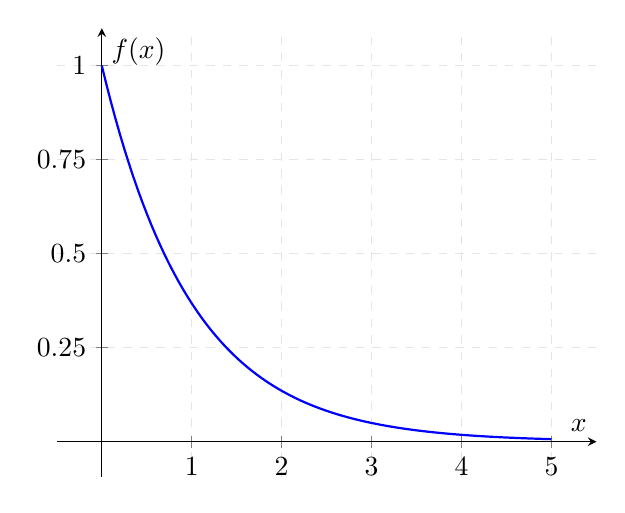
\begin{tikzpicture}
        \begin{axis}[
            domain=0:5,
            samples=100,
            axis x line=middle,
            axis y line=middle,
            xlabel={$x$},
            ylabel={$f(x)$},
            xtick={1,2,3,4,5},
            ytick={0.25, 0.5, 0.75,1},
            grid=major,
            grid style={dashed, gray!20},
            enlargelimits=true,
            %title={Exponential Distribution: $\lambda e^{-\lambda x}$ for $\lambda = 1$}
        ]
        \addplot[blue, thick] {exp(-x)};
        \end{axis}
    \end{tikzpicture}
    \source{ and processing: author}
\end{figure}

\begin{koment}
    Jak se exponencialni rozdeleni tyka BL? 

    Benfordovo rozdeleni muze pripominat exponencialni rozdeleni, proto bych mela popsat, jak to rozdeleni vypada, nakreslit nejaky pekny grafik a popsat co dela parametr lambda. Mozna by se hodil nejaky pekny priklad pouziti? 

    Mozna me jeste napada, jestli sem nenapsat co je to rozdeleni, frekventisticka definice pravdepodobnosti (since pocitam relativni frekvence vyskytu cislic na dane pozici a prirovnavam to k pravdepodobnostem) 
\end{koment}

Kdyz porovname exponencialni rozdeleni a rozdeleni podle benfordova zakona, narazime na dve vyrazne odlisnosti 
Benforduv zakon je diskretni (relativni frekvence pro jednotlive cislice), exponencialni rozdeleni je spojite. Dal, Benforduv zakon ma vetsi tails (jestli se tomu da vubec tak rikat pro diskretni rozdeleni), zatimco exponencialni rozdeleni ma tails velmi male. Pri zvoleni parametru, aby si byla rozdeleni blizka, vidime, jak jsou si odlisna. 

\begin{figure}[h]
    \centering
    \caption{Porovnani BL a Exp(0.45)}
    \label{fig:Exp0.45aBL}
    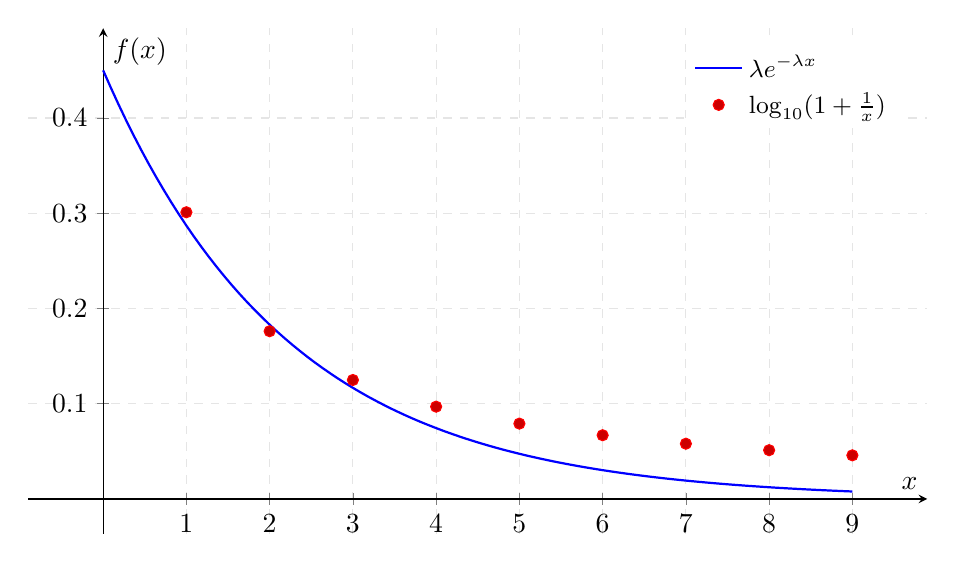
\begin{tikzpicture}
        \begin{axis}[
            width=13cm,  % Set the width of the plot
            height=8cm,  % Set the height of the plot
            domain=0:9,
            samples=100,
            axis x line=middle,
            axis y line=middle,
            xlabel={$x$},
            ylabel={$f(x)$},
            xtick={1,2,3,4,5,6,7,8,9},
            yticklabel style={/pgf/number format/.cd, fixed, precision=2}, 
            %ytick=\empty, 
            grid=major,
            grid style={dashed, gray!20},
            enlargelimits=true,
            %title={Porovnani BL a Exp(0.45)},
            legend style={draw=none, font=\small, cells={anchor=west}},
            legend pos=north east
        ]
        \addplot[blue, thick] {0.45*exp(-0.45*x)};
        \addlegendentry{$\lambda e^{-\lambda x}$}
        \addplot+[red, only marks, mark=*, mark size=2]
            coordinates {
            (1,0.3010) 
            (2,0.1761) 
            (3, 0.1249) 
            (4,0.0969) 
            (5,0.0791) 
            (6,0.0669) 
            (7,0.0580) 
            (8,0.0512) 
            (9,0.0458)
            };
        \addlegendentry{$\log_{10}(1 + \frac{1}{x})$}

        \end{axis}
    \end{tikzpicture}
    \source{ and processing: author}
\end{figure}


% %It is a non negative function, which sum equals to one. 

% For continuos variable is it defined as 

% \begin{equation}
%     P(x_1 \le X \le x_2) = \int\limits_{x_1}^{x_2} f (x) dx
% \end{equation}

% The distribution function is defined as 

% \begin{equation}
%     F(x) = P(X \le x), \quad \forall x \in R
% \end{equation}

% \begin{equation}
%     F(x) = \int\limits_{-\infty}^{x} f (t) dt, \quad -\infty <x<\infty
% \end{equation}

% \begin{koment}
%     neklesajici, v $-\infty$ je 0, v $\infty$ je 1

%     vymyslet jak to pojmout a propojit? 
% \end{koment}

\section{Hypothesis testing}

\subsection{First and second order errors (alpha beta)}

\subsection{P-value}

\subsection{Compliance to BL testing}

\subsubsection*{$\chi^2$ goodness of fit test}

To check the compliance of the data to the BL, we can use the $\chi^2$ goodness of fit test. The null hypothesis is that we assume the empirical distribution follows the theoretical BL distribution. The test criterion is given as such 

\begin{equation}
    \label{chi-sq-test}
    G= n \sum\limits_{d=1}^{9} \frac{(p_d -\pi_d)^2}{\pi_d} 
\end{equation}

\begin{align*}
    \text{where } &\pi_d \text{ is the theoretical frequency under BL distribution}, \\
    &p_d \text{ is the empirical frequency from the data, and} \\ 
    &n \text{ is the sample size}
\end{align*} 

as recommended in \citeauthor{Hronova2023}, \citeyear{Hronova2023} and  \citeauthor{kossovsky2014benford}, \citeyear{kossovsky2014benford}. %asi i Kossovsky

% \begin{koment}
%     Pozor na stanovení N při testování pomocí chisq testu.
%     Je tam důležité odlišit, co je skutečně ta reálná populace - uvádí na příkladu, že populace mohou být sales revenue za celé čtvrtletí (57 tisíc záznamů) - unique price list, unique products... ale třeba sales revenue z malého coffee shopu bude třeba k nějaké populaci přihodit - je zde možné testovat compliance a u toho velkého vzorku ne? Nevím, jestli to chápu dobře... 

%     Pokud ten dataset existuje sám o sobě in its unique fashion, je to potom comparison, ne compliance. Compliance to bude když testujeme (za použití statistického testu) nějaký náhodný výběr. (takže třeba hlasy jen pro jednoho z kandidátů?) 

%     Pak se dal ukazují Z testy (pro jednotlivá pozorování) a pak ChiSq test pro cele. Nakonec je pak jeste zajimava smerodnatna odchylka jako measure odlisnosti. 
% \end{koment}

\subsubsection*{Z test}

This test is performed individually on a particular digit/combination, however, the false positive error (type I) is more likely for the overall test of the chi-square.

Null hypothesis: Data obeys Benford's Law in the context of the particular digit/combination. % this individual observation obeys the benfords law ? 

\begin{equation}
    \label{z_test}
    Z_d = \frac{|P_o - P_e| - 1/2n}{\sqrt{(P_e(1-P_e)/n}}
\end{equation}

\begin{align*}
    \text{where } &P_o \text{ is the observed frequency of the particular digit/combination}, \\
    &P_e \text{ is the expected Benford proportion for the particular digit/combination, and} \\ 
    &n \text{ is the sample size}
\end{align*} 

We reject the null hypothesis when the $Z_d$ value is larger than $Z$ with the hladina významnosti alpha. $Z$ refers to the Standardized Normal Distribution, a Normal distribution with mean 0 and standard deviation 1. 

\subsubsection*{Kolmogorov-Smirnov test}

\section{Benford's Law Formulation}

The relative frequency of a leading digit approaches 

\begin{equation}
    \label{BZ-general_first}
\text{P(} X = d_i\text{)}= \log_{10}(1+1/d_i)
\end{equation}

where $d_i \in \{1,\dots,9\}$ for first digit law and $d_i \in \{10,\dots,99\}$ for the first-two digits law or even $d_i \in \{100,\dots,999\}$ for the first-three digits law. When plotted, it resembles nice logarithmic distribution, as seen on figure \ref{fig:FL}.  \cite{Cerqueti2202,Hronova2023,Newcomb1881}

\begin{figure}[h]
    \centering
    \caption{Theoretical frequencies of the first leading digits}
    \label{fig:FL}
    \pgfplotsset{width=8.5cm,compat=1.18}
        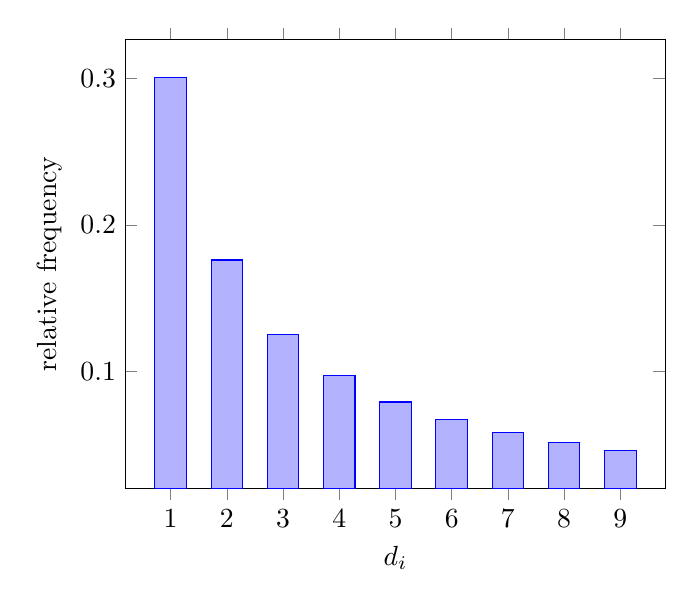
\begin{tikzpicture}
            \begin{axis}[
                ybar,
                bar width=.4cm,
                enlargelimits=0.1,
                ylabel={relative frequency},
                xlabel={$d_i$},
                symbolic x coords={1,2,3,4,5,6,7,8,9},
                xtick=data,
                ]
            \addplot coordinates {(1,0.3010) (2,0.1761) (3, 0.1249) (4,0.0969) (5,0.0791) (6,0.0669) (7,0.0580) (8,0.0512) (9,0.0458)};
            \end{axis}
        \end{tikzpicture}
    \source{ and processing: author}
\end{figure}

The first leading digit is the one found at the highest order and is non-zero. In the case of the number 124.857, the first digit would be 1, whereas for the number 0.03958, the first digit would be 3. According to Benford's law of the first digit, the theoretical frequencies correspond to the equation \ref{BZ-general_first}, indicating that the digit 1 occurs in the first position with a probability of 0.3, the digit 2 with 0.18, and so forth, with the digit 9 occurring with a probability of only 0.046.
%Compliance to this distribution is the first step in the nine-step procedure recommended by \citeauthor{kossovsky2014benford}, as mentioned in section \ref{correct_usage}.

As can be seen in the graph \ref{fig:FL}, the distribution is heavily skewed in favour of the lowest digits. As we move to the second (figure \ref{fig:second-digit-law}) and higher digits, this skew will flatten out significantly until there is no difference between the digits.  \cite{kossovsky2014benford}

This can be described by 

\begin{equation}
    \label{BZ-general_second}
    P(d) = \sum\limits_{k=1}^{9} \log_{10}\left( 1+\frac{1}{10k+d}\right), \quad \text{for } d = 0,1,\dots,9
\end{equation}

as mentioned by \citeauthor{Hronova2023} in \citeyear{Hronova2023}, assuming the independent occurence of the second leading digits. 

\begin{figure}[h]
    \centering
    \caption{Theoretical frequencies of the second leading digits}  
    \label{fig:second-digit-law}
        \pgfplotsset{width=8.5cm,compat=1.18}
            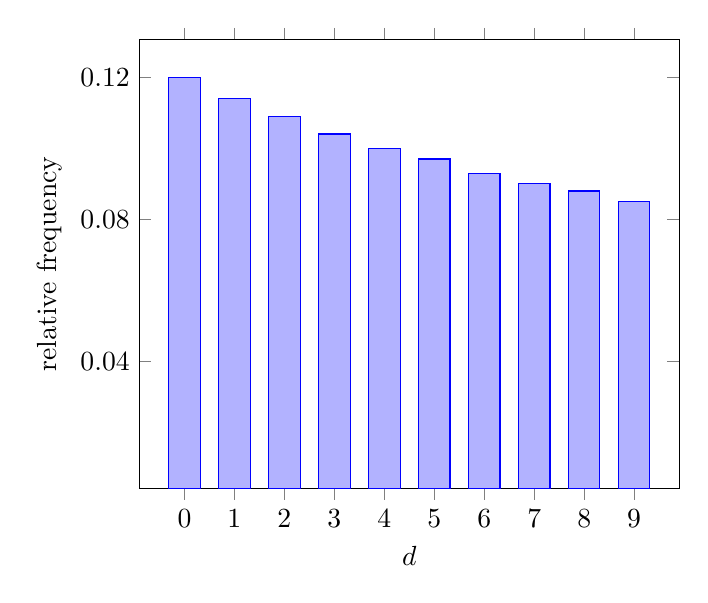
\begin{tikzpicture}
                \begin{axis}[
                    ybar,
                    bar width=.4cm,
                    ymin=0.015,
                    ytick={0.12, 0.08, 0.04},
                    enlargelimits=0.1,
                    ylabel={relative frequency},
                    xlabel={$d$},
                    symbolic x coords={0, 1,2,3,4,5,6,7,8,9},
                    xtick=data,
                    yticklabel style={/pgf/number format/fixed, /pgf/number format/precision=2},
                    ]
                \addplot coordinates {(0,0.12) (1,0.114) (2,0.109) (3, 0.104) (4,0.10) (5,0.097) (6,0.093) (7,0.09) (8,0.088) (9,0.085)};
                \end{axis}
            \end{tikzpicture}
    \source{: \citeauthor{kossovsky2014benford}, \citeyear{kossovsky2014benford}; processing: author}
\end{figure}

The distribution for the second digits is less skewed than that of the first leading digits. 
%Compliance to this distribution is the second step in the nine-step procedure recommended by \citeauthor{kossovsky2014benford}, as mentioned in section \ref{correct_usage}.
Coming to the third leading digit, the relative frequencies start to be close to equal as seen on figure \ref{fig:third-digit-law}. \cite{kossovsky2014benford}

This is explained by the following equation 

\begin{equation}
    P(d) = \sum\limits_{d_1=1}^{9} \sum\limits_{d_2=1}^{9} \dots \sum\limits_{d_{k-1}=1}^{9}   \log_{10}\left( 1+\frac{1}{\sum\limits_{i=1}^{k} d_i \cdot 10^{k-i} }\right), \quad \text{for } d_k = 0,1,\dots,9 
\end{equation}

describing third and following position relative frequencies, again with the assumption of independence of digit occurrences. And \uv{\emph{the Benford distribution converges to a uniform
multinomial distribution}} as put in \citeauthor{Hronova2023} in \citeyear{Hronova2023}. 

\begin{figure}[ht]
    \centering
    \caption{Theoretical frequencies of the third leading digits}  
    \label{fig:third-digit-law}
    \pgfplotsset{width=8.5cm,compat=1.18}
        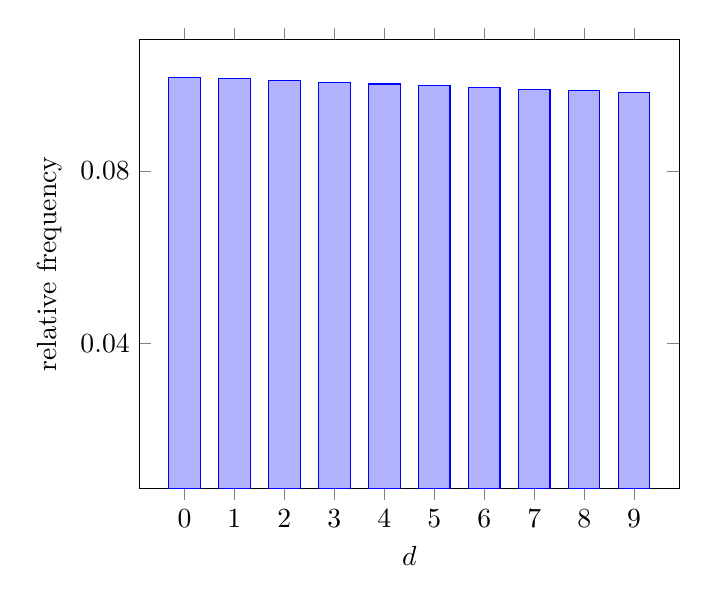
\begin{tikzpicture}
            \begin{axis}[
                ybar,
                bar width=.4cm,
                ymin=0.015,
                ytick={0.12, 0.08, 0.04},
                enlargelimits=0.1,
                ylabel={relative frequency},
                xlabel={$d$},
                symbolic x coords={0,1,2,3,4,5,6,7,8,9},
                xtick=data,
                yticklabel style={/pgf/number format/fixed, /pgf/number format/precision=2},
                ]
            \addplot coordinates {(0,0.1018) (1,0.1014) (2,0.1010) (3, 0.1006) (4,0.1002) (5,0.0998) (6,0.0994) (7,0.0990) (8,0.0986) (9,0.0983)};
            \end{axis}
        \end{tikzpicture}
    \source{: \citeauthor{kossovsky2014benford}, \citeyear{kossovsky2014benford}; processing: author}
\end{figure}

\subsection{Selected properties of numbers obeying Benford's Law}

\subsubsection{The Scale Invariance Principle of Benford's Law}

Given a dataset that already behaves according to BL, changing units (multiplying the whole dataset by the same constant) will still behave according to BL. Any arithmetic operation applied to the whole dataset does not change the underlying BL distribution. \cite{kossovsky2014benford, Hronova2023} %section 23 The Scale Invariance Principle 

\subsubsection{Digital Development Pattern}

Dividing the numbers by their orders into intervals such as (0.1,1), (1,10), (10,100) etc., we find that a pattern develops among them - the lower digits like 1 and 2 occur more frequently as the orders increase, while higher digits such as 8 and 9 gradually decrease in frequency. Data based on exponential growth should not be divided into intervals. \cite{kossovsky2014benford} % section 24

\begin{koment}
Comment on the conditions of what the dataset has to meet! 
%Aby BZ platil, musí být čísla - soubor čísel, takzvaně \emph{benfordovský} - dostatečně velký a splňovat podmínku \ref{BZ-podminka} \cite{kossovsky2014benford}. %section 10
\end{koment}

\subsection{Applicability of Benford's Law}

The law does not impose many conditions on the data that will be analysed, yet some must be met for reliable results. This section will discuss the following. 

\citeauthor{kossovsky2014benford} notes that for data to behave according to BL, its range should be wider, rather than narrow. He describes a measure \textbf{Order of Magnitude of Variability (OMV)} as:  

\begin{equation}
    OMV = \log(\text{90th percentile}) - \log(\text{10th percentile}) > 3 
    \label{OMV}
\end{equation}

and recommends it should be larger than 3. In practice, this means that our data should spread all the way from 1 to 10000 or more for consistent results. 
 
\subsubsection*{Correct usage} 

The compliance of our data with the law can be expected when only minimal conditions are met. Then the conformity can be tested. This makes the law good for detecting the presence of fraud or various manual manipulations of numbers with high accuracy. \cite{kossovsky2014benford, Cerqueti2202,kossovsky2014benford} 

When using Benford's Law to detect intentional fraud or data manipulation, the complete dataset is used, rather than a subset. Additionally, the dataset must satisfy conditions other than those mentioned in the previous chapters. The dataset should be large enough - for datasets with less than 100 observations, BL analysis is not recommended. %\cite{kossovsky2014benford} % section 26, strana 82
Only non-negative data should be used for analysis. For use in auditing, it is also recommended to eliminate small numbers, values less than, for example, 50, but that the portion removed be less than $10\%$. In addition, values that represent totals, summations, etc., should not be included if they come from the same sample. \cite{kossovsky2014benford} % section 27, strana 88 

\subsubsection*{Varying results from the expected distribution}

It is generally advisable to focus on deviations from the theoretical distribution in a given BL variation, specifically on the significantly higher values for the frequency of occurrence of a given digit. In graphical representation, these can be represented as spikes. There is minimal interest in the reduced frequencies, as any suspicious activity is likely to manifest itself through increased frequencies - when counting frequencies, an increase in one digit is much more detectable, with all other frequencies dropping slightly. \cite{kossovsky2014benford} % section 26, strana 85 

% \begin{koment}
%     grafický příklad jak vypadá hrot jakožto odchylka od konformity s BZ - pokud nebudu mít nic svého, Kossovsky strana 83. Potom i další ukázky podivných situací.
% \end{koment}

%There will always be variation, because few datasets are $100\%$ \textit{Benfordian}.  \cite{kossovsky2014benford} % section 26, strana 84

Deviance is to be expected, but where should the line be drawn?  \citeauthor{kossovsky2014benford} suggests distinguishing between two terms: compliance and comparison. When researching the data's compliance with BL, the data is expected to follow the logarithmic distribution very closely, the focus is on detecting manipulation, and if there is, whether it is random or structural. For comparison, the conditions are much looser. We don't assume any \textbf{prior population type (logarithmic distribution)}. For our use, we will be assuming the data should follow the distribution and therefore observe data compliance.


Next, the deviations should not show signs of any systematic error or pattern. Some pattern may emerge by rounding numbers, for example. The practice of rounding data is prevalent in the context of accounting, where values ending in 00 or 50 are frequently observed. This rounding process, which is often employed to streamline computations, can give rise to manipulation of higher orders while being harmless in context. Empirical evidence supports the prevalence of these values in practice. %\cite{kossovsky2014benford} %section 27, strana 92
However, such manipulations are unacceptable in, for example, electoral statistics, where votes simply cannot be rounded.
\cite{kossovsky2014benford}

% \begin{koment}
%     * insert příklad z analýzy volebních výsledků v Rusku, kde se zaokrouhlovalo, nebo odkaz na vyssi kapitolu kde se k tomu snad dostanu * 
% \end{koment}

There are also numbers that someone must have made up at some point. In accounting, donations are a good example. That is a number that someone has determined. Just as, for example, prizes. Such numbers do not follow BL and will show high degrees of deviation. \cite{kossovsky2014benford}

Alternatively, the validity of BL can be influenced by changed external situations in regards to the data itself. For instance, how does sales data follow BL distribution when affected by the pandemic in 2020? This has been answered by \citeauthor{Hronova2023} in \citeyear{Hronova2023}. Changes like this should be taken into account, and analysis should be adapted accordingly.


\subsection{Forensic digital analysis tests}

When detecting similar errors, it is often not enough to only look at the first digits' distribution. It is advised to look at the last two digits to detect rounding. For a comprehensive analysis, \citeauthor{kossovsky2014benford} recommends following tests:

\begin{enumerate}
    \item First-digits distribution
    \item Second-digits distribution
    \item Combination of the first-two-digits distributions
    \item Combination of the first-three-digits distributions
    \item Combination of the last-two-digits distributions 
    \item Examination of first-order digital development
    \item Examination of second-order digital development
    \item Value repetition test
    \item Observing the Digital Development and BL Pattern among it 
    \item Summation test   
\end{enumerate}

These tests, as they are generally very important to include, do not make any sense in our analysed data. Value repetition test is advised to be useful for data from the accounting or financial sector, digital development is not interesting since the election districts are set to be a particular size and summation test is not making any sense to be used in election analysis. 

% \subsubsection*{Combination of distributions}

\begin{koment}
    Popravdě, mám chuť toto skipnout, Summation test mi nedává v kontextu voleb až takový smysl, myslím, že ho vynechám. Value repetition test je doporučen pro accounting a financial data. Digital development je essential, na ten se musím podívat.  

    Jenže u toho je problém v tom, že volební okrsky jsou fixed na 1000 obyvatel, tudíž ten development nebude moc velkej. Co okresní data? Mám pocit, že se to mé práce taky úplně netýká. 
\end{koment}


\subsubsection*{Examination of a digital development}

Digital development pattern refers to the way distributions of digits evolve across different ranges of data. This pattern is observed in all random data sets, whether they follow Benford's Law or not. The pattern shows how the distribution of digits changes from lower to higher values of the data range. 

This pattern can only be seen when the data range is partitioned along integral powers of ten, such as (0.1, 1), (1, 10), (10, 100), etc. The pattern shows increasing skewness as you move from the left to the right of the data range. For smaller values, digit distributions are more equal. In the centre, the distribution becomes more logarithmic. For larger values, the distribution becomes highly skewed in favour of low digits. \cite{kossovsky2014benford}


% \subsubsection*{Value repetition test}

% \subsubsection*{Summation test}




\section{Analysis workflow}

This is the proposed analysis workflow for this thesis: 


Preprocessing: 

\begin{enumerate}
    \item load data 
    \item clean data - remove summations and totals 
    \item extract digits for analysis into separate datasets (first, last, first two, last two) 
\end{enumerate}

Analysis itself: 

\begin{enumerate}
    \item[4.] Is data fit for applying BL? (velikost okrsku, min max vzdalenost a tak)
    \item[5.] First leading digits compliance to BL
    \item[6.] Last digits test (their relative frequency is from the Uniform distribution)
    \item[7.] Summation test 
    \item[8.] Value Repetition test
\end{enumerate}

\chapter{Application on Election Data} %of Benford's Law 

V nasledujicím segmentu budeme analyzovat výsledky prezidentských voleb v Rusku, u kterých se předpokládá nějaký fraud, ve Spojených státech, kde můžeme být svědky \textbf{gerrymanderingu}, akorát to asi není topic této práce, když koukáme na fraud perspektivou digits... takže by tam žádný fraud být nejspíš neměl. Dále nahlédneme do Estonska, kde mají zdigitalizovaný volební systém, dá se tam volit i přes mobil, země, ke které vzhlížíme co se digitalizace týče. No a naši pouť zakončíme prezidentskými volbami v Česku, kde opět neočekáváme nějaký závratný fraud.  


\section{Russia}
https://www.theguardian.com/news/datablog/2012/mar/05/russia-putin-voter-fraud-statistics


\section{USA} 


\section{Czechia Presidential elections in 2023}
priority 

\begin{koment}
VERBATIM, PŘEPSAT:

V České republice se opakovaně setkáváme s poukazy na nejrůznější vady volebního procesu. Běžně se můžeme dočíst o kupčení s hlasy, o podezřele vysokých počtech zneplatněných hlasů, hromadných účelových změnách trvalého bydliště před konáním komunálních voleb, účelovém svážení občanů k volebním místnostem , nedostatečné kontrole hlasovacích místností6 zejména v noci z pátka na
sobotu, nekvalitní práci volebních komisí apod. \cite{Lebeda2021}

Reakce ze strany
státu na tyto podněty však byla dlouhou dobu spíše vlažná. Opatření, která by tyto ne-
dostatky eliminovala, byla v minulosti přijímána dosti pomalu. Transparentnosti bychom přitom měli věnovat velkou pozornost, protože spolu s důslednější kontrolou voleb totiž mohou vést k vyšší důvěře v demokratický režim, k vyšší volební účasti a tím pádem i k vyšší
legitimitě volených orgánů. \cite{Lebeda2021}

Podezřelé: 
Rozdíl mezi vydanými a odevzdanými obálkami, podíl neplatných hlasů (špatně odevzdané hlasy), 100 \% využitých preferenčních hlasů (celostátní průměr je asi 12 \%), 100 \% účast... Toto často vede na špatnou práci volební komise. \cite{Lebeda2021}

Dalším problémem je to, že se volební komise málo obměňují, tudíž k těmto chybám může docházet opakovaně a systematicky. \cite{Lebeda2021}

\end{koment}



\section{Estonia?}
non priority 


co mi vyšlo 

}

{%
\pagestyle{plain}
\chapter*{Conclusion}
\addcontentsline{toc}{chapter}{Conclusion}

In the conclusion, the author summarizes the individual conclusions, analyses 
and interpretations. It is useful if the author concludes by acknowledging the 
limits of his/her work and possibilities of continuing the topic.

\begin{koment}

    Vyznam BL pro aplikaci v digital fraud detection pro volby 

    Jednoduchost implementace 

    Ceske prezidentske volby: 
    \begin{itemize}
        \item transparentni uz jen tim, ze je k datum snadny pristup na CZSO webovych strankach 
        \item no evidence of fraud 
        \item posudek od OBSE , jen ze mame zrusit trest za pomluvu :)))
    \end{itemize}

    Americke prezidentske volby: 
    \begin{itemize}
        \item decentralizace volebniho system, dela si to kazdy stat sam, tezke kdyz chci konkretni data 
        \item no evidence of large scale fraud 
        \item posudek od OBSE
    \end{itemize}

    Beloruske prezidentske volby: 
    \begin{itemize}
        \item netransparentni
        \item multiple evidences of fraud 
        \item Voice, Zubr, Honest People dobra peace   
        \item vsichni vedi, ze v Belorusku si prezidenta proste nezvolis 
    \end{itemize}

    Limity digital detection of fraud 

    Other types of fraud

    Rozsireni (correlation among variables a tak) 

\end{koment}
}

%%% Seznam použité literatury
%%% Bibliography
\include{bibliography}

%%% Přílohy k práci, existují-li. Každá příloha musí být alespoň jednou
%%% odkazována z vlastního textu práce. Přílohy se číslují.
%%% Attachments to thesis, if any. Each attachment must be referenced at 
%%% least once in your own text. The appendices are numbered.
\part*{\Prilohy\thispagestyle{empty}}
\appendix
\chapter{Additional outputs of analysis of the Czech presidential election in 2023}


\begin{figure}[h]
    \centering
    \caption{First two digits distribution, Czechia 2023}
    \includegraphics[width=0.99\linewidth]{BT-DT-eng/fig/CZ23-both-first_two_digits.pdf}
    \label{fig:CZ23-both-first_two_digits}
\end{figure}

\begin{figure}[h]
    \centering
    \caption{Second digit distribution, Czechia 2023}
    \includegraphics[width=0.99\linewidth]{BT-DT-eng/fig/CZ23-both-second_digits.pdf}
    \label{fig:CZ23-both-second_digits}
\end{figure}

\begin{figure}[h]
    \centering
    \caption{Third digit distribution, Czechia 2023}
    \includegraphics[width=0.99\linewidth]{BT-DT-eng/fig/CZ23-both-third_digits.pdf}
    \label{fig:CZ23-both-third_digits}
\end{figure}

\begin{figure}[h]
    \centering
    \caption{Last digit distribution, Czechia 2023}
    \includegraphics[width=0.99\linewidth]{BT-DT-eng/fig/CZ23-both-last_digits.pdf}
    \label{fig:CZ23-both-last_digits}
\end{figure}

\begin{figure}[h]
    \centering
    \caption{First two digits distribution, Czechia 2023}
    \includegraphics[width=0.99\linewidth]{BT-DT-eng/fig/CZ23-dual-first_two_digits.pdf}
    \label{fig:CZ23-dual-first_two_digits}
\end{figure}

\begin{figure}[h]
    \centering
    \caption{Third digits distributions from both candidates in Czechia in 2023}
    \includegraphics[width=0.99\linewidth]{BT-DT-eng/fig/CZ23-dual-third_digits.pdf}
    \label{fig:CZ23-dual-third_digits}
\end{figure}








\chapter{Additional outputs of analysis of the USA presidential election in 2024}

% \begin{figure}[h]
%     \centering
%     \caption{First digit distribution, total votes, USA 2024}
%     \includegraphics[width=0.99\linewidth]{BT-DT-eng/fig/USA24-both-first_digits.pdf}
%     \label{fig:USA24-both-first_digits}
% \end{figure}

% \begin{figure}[h]
%     \centering
%     \caption{First two digits distribution, total votes, USA 2024}
%     \includegraphics[width=0.99\linewidth]{BT-DT-eng/fig/USA24-both-first_two_digits.pdf}
%     \label{fig:USA24-both-first_two_digits}
% \end{figure}

% \begin{figure}[h]
%     \centering
%     \caption{Second digit distribution, total votes, USA 2024}
%     \includegraphics[width=0.99\linewidth]{BT-DT-eng/fig/USA24-both-second_digits.pdf}
%     \label{fig:USA24-both-second_digits}
% \end{figure}

% \begin{figure}[h]
%     \centering
%     \caption{Third digit distribution, total votes, USA 2024}
%     \includegraphics[width=0.99\linewidth]{BT-DT-eng/fig/USA24-both-third_digits.pdf}
%     \label{fig:USA24-both-second_digits}
% \end{figure}

% \begin{figure}[h]
%     \centering
%     \caption{Last digit distribution, total votes, USA 2024}
%     \includegraphics[width=0.99\linewidth]{BT-DT-eng/fig/USA24-both-last_digits.pdf}
%     \label{fig:USA24-both-last_digits}
% \end{figure}

\begin{figure}[h]
    \centering
    \caption{First two digits distribution from both candidates, USA 2024}
    \includegraphics[width=0.99\linewidth]{BT-DT-eng/fig/USA24-dual-first_two_digits.pdf}
    \label{fig:USA24-dual-first_two_digits}
\end{figure}

\begin{figure}[h]
    \centering
    \caption{Third digits distributions from both candidates, USA 2024}
    \includegraphics[width=0.99\linewidth]{BT-DT-eng/fig/USA24-dual-third_digits.pdf}
    \label{fig:USA24-dual-third_digits}
\end{figure}








\chapter{Additional outputs of analysis of the Belarussian presidential election in 2020}


\begin{figure}[h]
    \centering
    \caption{First two digits distribution, Belarus 2020}
    \includegraphics[width=0.99\linewidth]{BT-DT-eng/fig/BLR20-all-first_two_digits.pdf}
    \label{fig:BLR20-all-first_two_digits}
\end{figure}

\begin{figure}[h]
    \centering
    \caption{Second digit distribution, Belarus 2020}
    \includegraphics[width=0.99\linewidth]{BT-DT-eng/fig/BLR20-all-second_digits.pdf}
    \label{fig:BLR20-all-second_digits}
\end{figure}

\begin{figure}[h]
    \centering
    \caption{Third digit distribution, Belarus 2020}
    \includegraphics[width=0.99\linewidth]{BT-DT-eng/fig/BLR20-all-third_digits.pdf}
    \label{fig:BLR20-all-third_digits}
\end{figure}

\begin{figure}[h]
    \centering
    \caption{Last digit distribution, Belarus 2020}
    \includegraphics[width=0.99\linewidth]{BT-DT-eng/fig/BLR20-all-last_digits.pdf}
    \label{fig:BLR20-all-last_digits}
\end{figure}

\begin{figure}[h]
    \centering
    \caption{First two digits distribution, Belarus 2020}
    \includegraphics[width=0.99\linewidth]{BT-DT-eng/fig/BLR20-dual-first_two_digits.pdf}
    \label{fig:BLR20-dual-first_two_digits}
\end{figure}

\begin{figure}[h]
    \centering
    \caption{Third digits distributions from all candidates, Belarus 2020}
    \includegraphics[width=0.99\linewidth]{BT-DT-eng/fig/BLR20-dual-third_digits.pdf}
    \label{fig:BLR20-dual-third_digits}
\end{figure}








\chapter{Source code used}

\begin{code}{R}{Libraries used}{lib}
library(readr)
library(stringr)
library(dplyr)
library(ggplot2)
library(tidyr)
library(patchwork)
\end{code}

\end{document}
